\documentclass{article}
\usepackage{graphicx}
\begin{document}
\section{Introduction}
Simple Task Log is a web application, working in all modern browsers, providing functionality for simple tasks management. Each task has a unique name, deadline and a flag whether it's completed or not.
\section{UI}
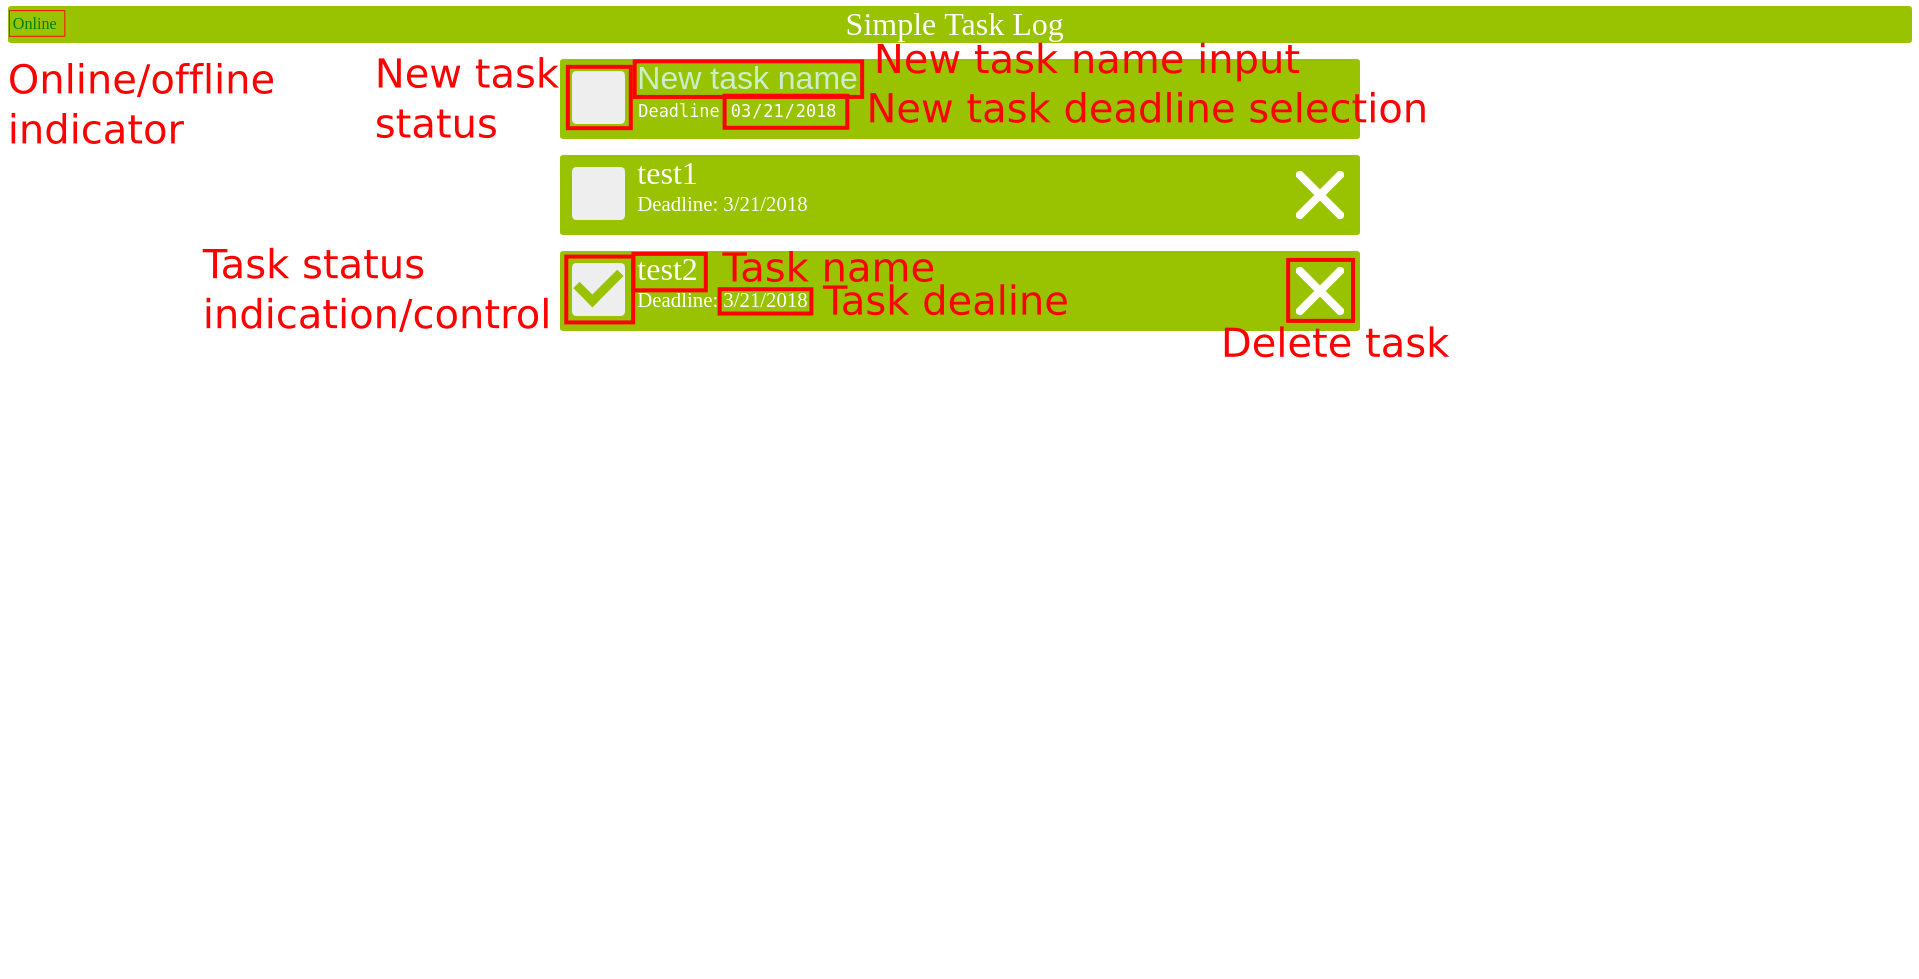
\includegraphics[width=\textwidth]{ui}
As shown on the screenshot, application has several main parts:
\subsection{Header}
Header is a bar on the top of the page, displaying the application's name and a network connectivity status (whether the application is working online, in which case the indicator says so in green or offline, which would be indicated by the red text).
\subsection{New task prompt}
New task prompt consists of three fields - name input, completion flag checkbox and deadline date selector (which has the current date as a default value). To create a task, you type in a name and press Enter. After that the application checks if you have correctly entered a deadline and a name (which cannot be the same as the name of any of the previous tasks). In case the constraints are satisfied, a new task is created and displayed in the task list. Otherwise, you hear an alarm and see a warning with an information about what was wrong.
\subsection{Task list}
Task list displays the list of the previously created tasks and allows to delete a task, or alter it's completion flag. On mouse hover a list entry is upscaled.
\section{History}
You can always traverse the history of your changes by traversing the page history in your browser. Task creation, deletion and changing completion status are considered history checkpoints.
\section{Print}
You can print the webpage, in which case everything, but the header and the task list will be hidden, and everything shown will be styled for print.
\end{document}
